\chapter{Datasets}
To test our extraction-classification pipeline, we use four progressively more complex datasets. We start by classifying simple 2D shapes, then move on to simple 3D shapes, and last, we attempt to classify a dataset of real photographs of cats and dogs.

\section{2D Shapes Dataset}
For the simplest dataset, we use a four shapes dataset \cite{kaggleFourShapes}. The dataset contains $16000$ images of four shapes: square, star, circle, and triangle. The dataset was created from poster board cutouts of the shapes, painted green. While rotating, each shape was recorded using a Garmin Virb 1080p action camera for two minutes. Shapes were then cropped out from the frames of the video and resized to $200\times200$ pixels. The green color of the cutouts in frames is then changed to a pure black color, while the rest of the image is changed to a pure white color. An example of the data can be seen in \figref{fig:four_shapes}.

As we are doing a binary classification, we use only the pair of a circle and a star.
\begin{figure}[ht]
    \centering
    \begin{subfigure}[t]{0.2\textwidth}
        
\includegraphics[width=\textwidth]{Figures/datasets/circle.png}
        \caption{Circle}
    \end{subfigure}
    \begin{subfigure}[t]{0.2\textwidth}
        
\includegraphics[width=\textwidth]{Figures/datasets/star.png}
        \caption{Star}
    \end{subfigure}
    \caption[Photographs of a circle and a star from the Four Shapes dataset]{Photographs of a circle and a star from the Four Shapes dataset \cite{kaggleFourShapes}.}
    \label{fig:four_shapes}
\end{figure}

\section{3D Shapes Dataset}
The 3D Shapes dataset contains $20$ images of a box and $20$ images of a sphere from different points of view. The shapes are colored red, while the background is colored white. The objects are illuminated by a single light source, providing a nice and sharp shadow and shading of the each shape. The dataset was generated by Ing. Lukáš Pospíšil, Ph.D. in POV-Ray \cite{povray}. Each of the images is a $300\times200$ pixels. An example of each shape can be seen in \figref{fig:3d_shapes}.
\begin{figure}[ht]
    \centering
    \begin{subfigure}[t]{0.2\textwidth}
        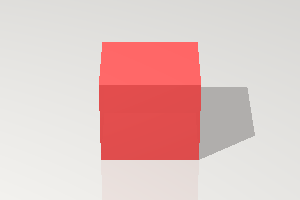
\includegraphics[width=\textwidth]{Figures/datasets/box.png}
        \caption{Box}
    \end{subfigure}
    \begin{subfigure}[t]{0.2\textwidth}
        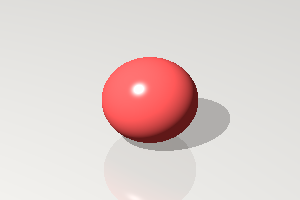
\includegraphics[width=\textwidth]{Figures/datasets/sphere.png}
        \caption{Sphere}
    \end{subfigure}
    \caption[3D shapes, generated by Ing. Lukáš Pospíšil, Ph.D. in POV-Ray]{3D shapes, generated by Ing. Lukáš Pospíšil, Ph.D. in POV-Ray \cite{povray}.}
    \label{fig:3d_shapes}
\end{figure}

\section{Cats and Dogs Dataset}
The Cats and Dogs dataset is created from the Oxford-IIIT Pet Dataset \cite{parkhi12a}. As the original dataset contains few damaged images, we use a fixed version of the dataset from \cite{ml4py_dataset}.
